\documentclass[11pt]{article}
\usepackage[a4paper, margin=1in]{geometry}
\usepackage{graphicx}
\usepackage{tabularx}
\usepackage{amsmath}
\usepackage{hyperref}
\usepackage{fontawesome}

\title{Vision assignment 2}
\author{sumanasekarawkgg.19 }

\begin{document}

\thispagestyle{empty}
\begin{center}
   \begin{figure}
   \vspace*{1.5cm}
       \centering
       
\includegraphics[width=4.8cm]{Images/uom.png}
   \end{figure}
   
   Department of Electronic and Telecommunication Engineering \\ University of Moratuwa \\
   \vspace{2cm}
   {\fontsize{14}{17}\selectfont\textbf{\\Assignment II\\}}
    \vspace{8cm}
    190610E - Sumanasekara W.K.G.G. 
   \vspace{3cm}
   \\This report is submitted as a partial fulfillment of module EN2550
   \vspace{0.5cm} \\
   \today
\end{center}

\newpage
\clearpage
\pagenumbering{arabic} 

\noindent \textbf{Note}: All codes relevant to this assignment can be found in \faGithub{ \url{https://github.com/GevinduGanganath/EN2550/tree/main/Assignment%202}}
\\

\noindent \textbf{Question 1}

\noindent In the first part of the assignment,  a circle is estimated using the RANSAC algorithm. Objective is to write a code for RANSAC manually.
Figure \ref{RANSAC code} shows the python code written by me. 
\begin{figure}[!h]
    \centering
    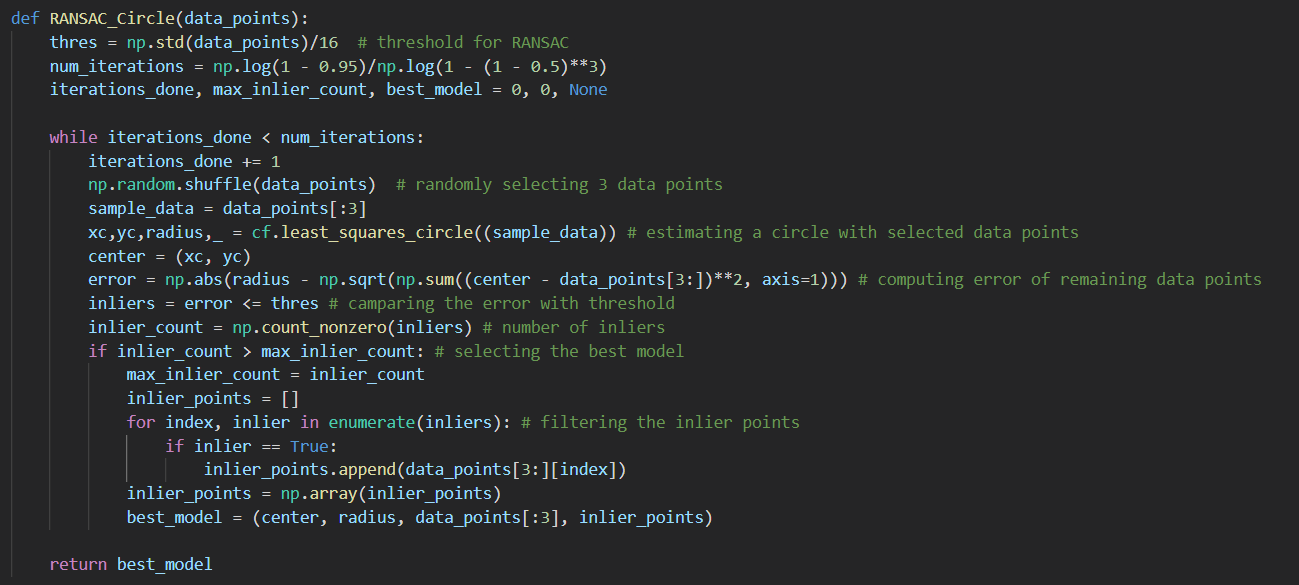
\includegraphics[width=0.8\textwidth]{Images/RANSAC code.PNG}
    \caption{Code snip of RANSAC algorithm}
    \label{RANSAC code}
\end{figure}

\noindent RANSAC parameters were set as follows:
\begin{itemize}
    \item Threshold: Standard deviation of data points divided by 16 (selected by trial and error)
    \item Number of samples (s): 3
    \item Probability (p): 0.95
    \item Outlier ration (e): 0.5
    \item Number of iterations $ = \frac{log(1-p)}{log(1-(1-e)^s)} \approx 22 $
\end{itemize}

\noindent Data points are shuffled at each iteration and the first three data points were selected to estimate the circle. \textit{least squares circle} 
function of the \textit{circle fit} python library was used to compute the center and radius. Then the distance between the center and the remaining 
data points are calculated. By comparing those values with the threshold we can count the number of inliers. The iteration which gives the highest
number of inliers was selected and using those inliers best model can be calculated. \\

\noindent Figure \ref{RANSAC} shows the results. Circle obtained by RANSAC algorithm (red) is giving better 
results than the inbuilt least square fitting function. 

\begin{figure}[!h]
    \centering
    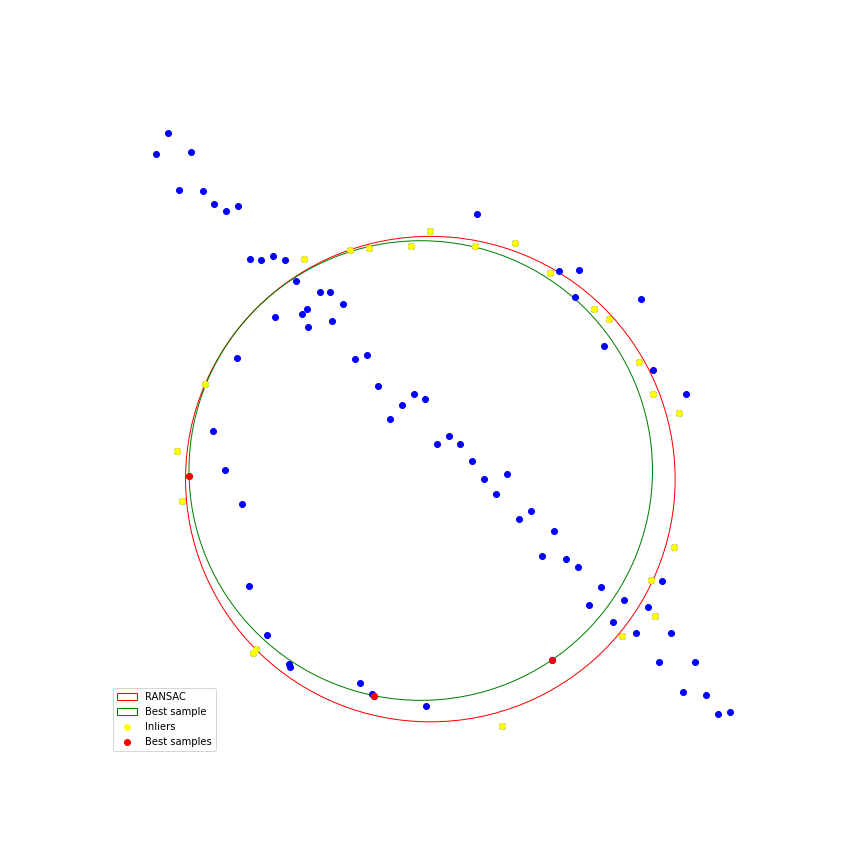
\includegraphics[width=0.8\textwidth]{Images/1.png}
    \caption{Results of RANSAC}
    \label{RANSAC}
\end{figure}


%\newpage
%\bibliographystyle{IEEEtran}
%\bibliography{ref}

\end{document}